% Theory part of the module.
%
% Module TH-37 of Section 6.7 of the syllabus: "Data, Algorithm, and
% Machine: the three places of a bottleneck. A method to find the bottleneck
% before you optimize." Type T, 25 minutes.
%
% Sources: the D·A·M taxonomy appendix of Volume I (the three axes, the
% intersections, the iron law mapping, the rules of thumb, the
% anti-patterns, and the three case studies), and section "D·A·M Taxonomy" of
% Volume I chapter 5 (the three axes as the alignment of the data, the
% algorithm, and the machine of a digit recognizer). No other source is used,
% so the credits frame names only the textbook.
%
% The numbers of this module have two origins. Each frame says so in its
% source line.
% 1. A number that a source reports: the screening thresholds of the
%    appendix, the case-study measurements, the ridge points of the
%    accelerators, and the latency example of chapter 5.
% 2. A value of this course: none. The module uses no measurement of the
%    course.
%
% Size: 8 to 12 frames for a recap module of 25 minutes.
%
% One figure is adopted from the sources: the roofline silhouette of the
% running example of Volume I, chapter 5. The other two diagrams are drawn
% again with TikZ. Rule 3 of ATTRIBUTION.md gives the source of the adopted
% figure and the change of each redrawn diagram.

% ------------------------------------------------------- 1. the symptom
\begin{frame}{A slow system does not name its cause}
  \small A device misses its deadline. The number is on the dashboard, and
  the team has one hour to act.
  \vskip 0.4em
  \begin{itemize}
    \item Three groups are in the room. One owns the sensors, one wrote the model,
          and one owns the chip.
    \item Each group has an improvement ready. None of them has a
          measurement.
  \end{itemize}
  \vskip 0.4em
  \keypoint{Optimizing before measuring picks a random axis and hopes.}
\end{frame}

% ----------------------------------------------------------- 2. the triad
\begin{frame}{Three axes, one system}
  \begingroup\centering
  \begin{tikzpicture}[font=\scriptsize, scale=0.86, transform shape,
      axis/.style={align=center, text width=1.5cm, inner sep=1pt,
                   font=\scriptsize\sffamily\bfseries, text=darkcyan},
      ovl/.style={align=center, text width=1.5cm, inner sep=1.5pt,
                  fill=white}]
    \draw[draw=coolgray, thick] (0,1.5) circle (1.45);
    \draw[draw=coolgray, thick] (-1.2,-0.9) circle (1.45);
    \draw[draw=coolgray, thick] (1.2,-0.9) circle (1.45);
    \node[axis] at (0,2.2)      {Algorithm};
    \node[axis] at (-1.85,-1.6) {Data};
    \node[axis] at (1.85,-1.6)  {Machine};
    \node[ovl] at (-0.78,0.62)  {what to\\learn from};
    \node[ovl] at (0.78,0.62)   {how to execute\\efficiently};
    \node[ovl] at (0,-1.32)     {how to move\\information};
  \end{tikzpicture}\par\endgroup
  \vskip 0.4em
  \small A change on one axis moves the constraint of the other two. That is
  why one number never tells the whole story.
  \vskip 0.3em
  \small Three words appear in the rest of this module. An
  \textbf{accelerator} is a separate chip that does the arithmetic of a
  model. A \textbf{FLOP} is one floating-point operation. A \textbf{byte} is
  one unit of data.
\end{frame}

% ------------------------------------------------------- 3. the axis table
\begin{frame}{What each axis controls}
  \footnotesize
  \begingroup\centering
  \begin{tabular}{@{}L{2.3cm}L{3.6cm}L{3.9cm}@{}}
    \toprule
    Axis & Its limit & Its high-leverage change \\
    \midrule
    Data & Volume, quality, arrival rate & Take less data, or better data \\
    Algorithm & Operations and dependencies & Compress the model \\
    Machine & Compute, memory, I/O & Change the hardware \\
    \bottomrule
  \end{tabular}\par\endgroup
  \vskip 0.5em
  \small Work on the Data axis alone and the load moves. Less data and
  cleaner labels raise the quality of the information, and they also cut the
  number of bytes that the Machine axis has to move.
\end{frame}

% -------------------------------------------------- 4. the pairwise zones
\begin{frame}{The interesting places are the overlaps}
  \begingroup\centering
  \footnotesize
  \begin{tabular}{@{}L{3.4cm}L{4.4cm}@{}}
    \toprule
    Zone & The question it asks \\
    \midrule
    Data alone & Is the information itself right? \\
    Algorithm alone & Is the logic right? \\
    Machine alone & Is the physics fast enough? \\
    Data and Algorithm & What can the model learn from this data? \\
    Data and Machine & Can the machine be fed fast enough? \\
    Algorithm and Machine & Does the code execute this logic well? \\
    All three at once & Is this a system, and is it measured? \\
    \bottomrule
  \end{tabular}\par\endgroup
  \vskip 0.5em
  \small A single-axis problem is rare. Most slow systems sit on a boundary,
  and a change on one side of a boundary moves the load to the other side.
\end{frame}

% ------------------------------------------------------- 5. the iron law
\begin{frame}{Time is three terms}
  \begin{equation*}
    T = \underbrace{\frac{D_{\text{vol}}}{\text{BW}}}_{\text{data term}}
      + \underbrace{\frac{O}{R_{\text{peak}} \cdot \eta_{\text{hw}}}}_{\text{compute term}}
      + \underbrace{L_{\text{lat}}}_{\text{latency term}}
  \end{equation*}
  \small
  \begin{itemize}
    \item The data term counts the bytes and the bandwidth that move them.
    \item The compute term counts the operations, the peak rate of the
          hardware, and how much of that rate the run reaches.
    \item The latency term is the fixed cost of launching, waiting, and
          synchronizing.
  \end{itemize}
  \vskip 0.2em
  \small The three terms are the three axes in units of seconds. The largest
  one is the part that costs the time.
\end{frame}

% ---------------------------------------------------- 6. the dominant term
\begin{frame}{The largest term names the axis}
  \footnotesize
  \begin{tabular}{@{}L{2.9cm}L{3.5cm}L{3.6cm}@{}}
    \toprule
    If the run is & Then fix & Do not bother with \\
    \midrule
    Memory bound & Quantize, prune, fuse, batch & A faster arithmetic unit \\
    Compute bound & Better kernels, lower precision & More bandwidth \\
    Latency bound & Shorter chain, fewer launches & Any extra compute \\
    \bottomrule
  \end{tabular}
  \vskip 0.5em
  \small To \textbf{quantize} is to store a number in fewer bits. To
  \textbf{prune} is to drop weights. To \textbf{fuse} is to join two
  operations, so that the data between them moves once. \textbf{Batching}
  sends several inputs at once, so one weight read serves all of them.
  \vskip 0.3em
  \small The last column is the expensive column. A faster accelerator does
  nothing for a workload that waits for its data.
\end{frame}

% ------------------------------------------------------- 7. the ridge point
\begin{frame}{One number separates memory from compute}
  \begin{columns}[T]
    \begin{column}{0.40\textwidth}
      \centering
      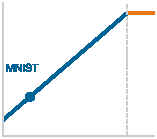
\includegraphics[height=3.9cm]{images/modules/TH-37/vol1_nn_computation_margin_004.pdf}
    \end{column}
    \begin{column}{0.56\textwidth}
      \small
      \begin{itemize}
        \item The arithmetic intensity of a workload is its operations per
              byte moved.
        \item The ridge point of a chip is its peak rate divided by its
              bandwidth. For a server accelerator it sits between 150 and
              300 FLOP per byte.
        \item Below the ridge the workload is memory bound. Above it, the
              workload is compute bound.
      \end{itemize}
    \end{column}
  \end{columns}
  \vskip 0.3em
  \small The dot on the slope is a small MNIST digit classifier, and it needs
  about 12 FLOP for each byte it moves. That is more than ten times below the
  ridge point, so it stays on the slope even on a large accelerator.
  \source{Figure adopted from Volume I, chapter 5.}
\end{frame}

% ------------------------------------------------------ 8. the screen rules
\begin{frame}{Read the dashboard before you touch the code}
  \footnotesize
  \begingroup\centering
  \begin{tabular}{@{}L{4.6cm}L{4.6cm}@{}}
    \toprule
    The reading & What it usually means \\
    \midrule
    Accelerator under 80 percent busy & Data, host, or launch starvation \\
    Accelerator over 95 percent busy & Compute bound, unless the memory
      bus is also full \\
    Batch size of one & Latency, not throughput, is the goal \\
    Data wait above 10 percent of a step & The pipeline, not the model \\
    Model FLOP utilization under 30 percent & The work of the model itself is
      small next to the work of the run \\
    \bottomrule
  \end{tabular}\par\endgroup
  \vskip 0.4em
  \small \textbf{Batch size} is the number of inputs the model handles at one
  time. \textbf{Model FLOP utilization} is the rate the model reaches,
  divided by the peak rate of the accelerator.
  \vskip 0.3em
  \small These are screens, not proofs. Each one names the measurement that
  confirms it.
\end{frame}

% ------------------------------------------------------------ 9. the traps
\begin{frame}{Three ways to optimize the wrong axis}
  \small
  \begin{itemize}
    \item \textbf{The hardware crutch.} A faster accelerator is bought for a
          slow data loader. The new chip waits faster.
    \item \textbf{The model twiddle.} The architecture is changed while the
          bottleneck sits in the disk or in the network.
    \item \textbf{The premature optimizer.} A custom kernel is written while
          the model still repeats the same operation twice.
  \end{itemize}
  \vskip 0.4em
  \small A \textbf{kernel} is the compiled code that runs one operation on
  the accelerator.
  \vskip 0.3em
  \small The three traps have one cause: acting before the measurement.
\end{frame}

% --------------------------------------------------------- 10. the cases
\begin{frame}{Three cases, three axes}
  \footnotesize
  \begingroup\centering
  \begin{tabular}{@{}L{3.9cm}L{2.4cm}L{2.9cm}@{}}
    \toprule
    Symptom & Axis & The move that follows \\
    \midrule
    Accelerator between 10 and 40 percent, and gaps while it waits & Data &
      Decode each input once, and send the result early \\
    20 ms budget missed at batch size one & Algorithm and Machine &
      Shorten the chain, or quantize the weights \\
    Accelerator at 99 percent, memory bus idle & Machine &
      Lower the precision, or add a bigger chip \\
    \bottomrule
  \end{tabular}
  \par\endgroup
  \vskip 0.4em
  \small The same reading of the dashboard sends two of these cases to
  different teams.
\end{frame}

% ---------------------------------------------------------- 11. the method
\begin{frame}{The method in four passes}
  \begingroup\centering
  \begin{tikzpicture}[font=\scriptsize, >=stealth, scale=0.94,
      transform shape,
      bx/.style={draw=coolgray, rounded corners=2pt, fill=boxgray,
                 align=center, text width=2.15cm, minimum height=0.9cm}]
    \node[bx] (a) at (0,0)      {Write the\\ missed target};
    \node[bx] (b) at (2.6,0)    {Pick the\\ candidate axis};
    \node[bx] (c) at (5.2,0)    {Measure the\\ one term};
    \node[bx] (d) at (7.8,0)    {Change it,\\then measure again};
    \draw[->] (a) -- (b);
    \draw[->] (b) -- (c);
    \draw[->] (c) -- (d);
    \draw[->, cardinalred, dashed] (d.south) -- ++(0,-1.0)
      -| (a.south);
    \node[font=\scriptsize, text=cardinalred, align=center, fill=white,
          inner sep=2pt] at (3.9,-1.22)
      {no change? the axis was wrong};
  \end{tikzpicture}\par\endgroup
  \vskip 0.5em
  \small The loop is the method. The label of the axis is a hypothesis, and
  the last pass is the only one that settles it.
\end{frame}

% ------------------------------------------------------------ 12. the recap
\begin{frame}{What to remember}
  \small
  \begin{enumerate}
    \item Three axes: Data, Algorithm, and Machine. A change on one moves
          the constraint of the other two.
    \item Time is three terms: the bytes over the bandwidth, the operations
          over the peak rate, and the fixed latency. The largest term names
          the axis.
    \item The last column of the diagnostic table is the expensive one.
    \item The axis is a hypothesis. The measurement settles it.
  \end{enumerate}
  \vskip 0.3em
  \keypoint{Name the bottleneck before you optimize it.}
\end{frame}

% ------------------------------------------------------------- exercise
\exerciseframe{Name the bottleneck}{A team has three slow systems.
\begin{enumerate}
  \item A speech service on a fast accelerator answers in 340 ms, and the
        accelerator is idle 60 percent of the time. A log of the run shows
        the gaps, and the audio files are decoded during them.
  \item A camera on a microcontroller runs the same network in 95 ms. The
        same network runs in 12 ms on a laptop, and the two use the same
        number of operations.
  \item A training job uses a new accelerator with twice the arithmetic of
        the old one. The step time falls by 4 percent.
\end{enumerate}

For each system, name the bottleneck and give the one measurement that would
confirm it.
}

\answerframe{Name the bottleneck}{
  \begin{enumerate}
    \item \textbf{Data.} The accelerator is idle because it waits for
          decoded audio. The confirming measurement is the data wait time
          against the step time. Adding arithmetic changes nothing.
    \item \textbf{The Data and Machine boundary.} The same work on a
          different machine finishes eight times faster, so the arithmetic
          was not the limit: the run was memory bound. The confirming
          measurement is the arithmetic intensity against the ridge point
          of each machine.
    \item \textbf{The Data and Machine boundary.} Twice the arithmetic gave
          4 percent, so the arithmetic was not the binding term. The
          confirming measurement is the arithmetic intensity of the job
          against the ridge point of the new accelerator. Below the ridge,
          the extra arithmetic sat unused.
  \end{enumerate}
  \vskip 0.3em
  \small Two of the three cases point at the data term. That is the usual
  result, and it is why the first measurement is a wait time and not a
  speed number.
}